
\chapter{Aplikace v konkrétních rodinách distribucí}

V této kapitole použijeme minimální Rényiho odhady ({\mRao}y) v různých rozděleních pravděpodobnosti. Výsledky pro normální rozdělení byly uvedeny již v \cite{Demut2010}. My jsem se tedy zaměřili na exponenciální, Laplaceovo, Cauchyho a Weibullovo rozdělení pravděpodobnosti. V případě těchto rodin jsme se snažili o odvození konkrétního tvaru odhadu podle \eqref{Renyi-estimator_formula} a také tvaru influeční funkce \eqref{IF}.

\section{Laplaceovo rozdělení pravděpodobnosti} %%%%%%%%%%%%%%%%%%%%%  LAPLACE   %%%%%%%%%%%%%%%%%%%%%%

Zde použijeme min $\mathfrak{R}_\alpha$-odhady k odhadu parametru $\theta = (\mu,\lambda)$ pro případ Laplaceova rozdělení. Hustota pravděpodobnosti má tedy tvar
\begin{equation}
	p_\theta = \frac{1}{2\lambda} e^{-\frac{|x-\mu|}{\lambda}}, \qquad \mu\in \mathbb{R},\, \lambda>0.
\end{equation}
Pro $\alpha = 0$ se odhad rovná maximálně věrohodnému odhadu 
\begin{eqnarray}
	\theta_{\alpha,n} & = & \arg \max_{\theta \in \Theta} \frac{1}{n} \sum^n_{i=1} \ln \left[ \frac{1}{2\lambda}\exp \left[-\frac{|x_i-\mu|}{\lambda} \right] \right] \nonumber \\
	& = & \arg \max_{\theta \in \Theta} \left[ \ln \frac{1}{2\lambda} - \frac{1}{n} \sum^n_{i=1} \frac{|x_i-\mu|}{\lambda} \right].
\end{eqnarray}
Podmínka \ref{beta-podminka} platí pro každé $\beta>0$, takže pak pro $\alpha>0$ můžeme  min $\mathfrak{R}_\alpha$-odhad \eqref{Renyi-estimator_formula} pro Laplaceovo rozdělení psát jako 
\begin{equation}
	\theta_{\alpha,n} = \arg \max_{\theta \in \Theta} \left[ (2\lambda)^{-\frac{\alpha}{1+\alpha}} \frac{1}{n} \sum_{i=1}^n \exp \left[-\alpha\frac{|x_i-\mu|}{\lambda} \right] \right].
\end{equation}

\noindent Nyní spočítáme influenční funkci podle \eqref{IF}. Položíme-li odhadovaný parametr $\theta = \mu$ při známém $\lambda = 1$, pak nám vychází 
\begin{equation}
	\mathrm{IF}(x;T_{\mathfrak{R}_\alpha},\mu) = (1+\alpha )^{\frac{3}{2}} (x-\mu )  e^{-\frac{\alpha}{2} (x-\mu )^2}. % IF(x,mu)
	\label{IF-laplace-mu}
\end{equation}
Pokud prohodíme úlohu parametrů, tedy pokud bude hledaným parametrem $\theta = \lambda$ a $ \mu := 0$ bude známe, vychází 
\begin{equation}
	\mathrm{IF}(x;T_{\mathfrak{R}_\alpha},\lambda) = (1 + \alpha)^2 \left(-\lambda + (1 + \alpha)|x|\right)  e^{-\frac{\alpha|x|}{\lambda}}	. % IF(x,sigma)
	\label{IF-laplace-lambda}
\end{equation}

\begin{figure}[htb]
\begin{center}
\begin{tabular}{c c c}
	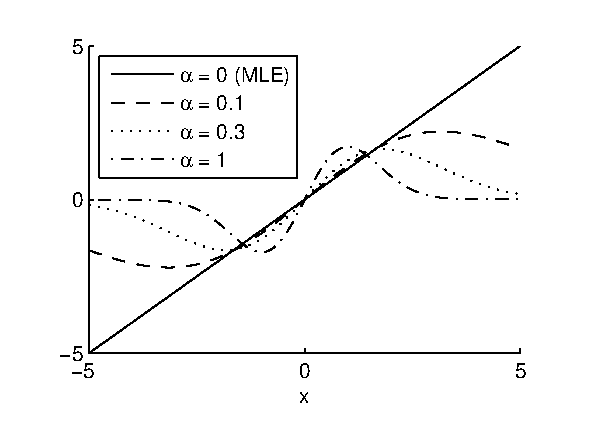
\epsfig{file=Laplace-IF-mu.eps, height=2in} 
	&&
	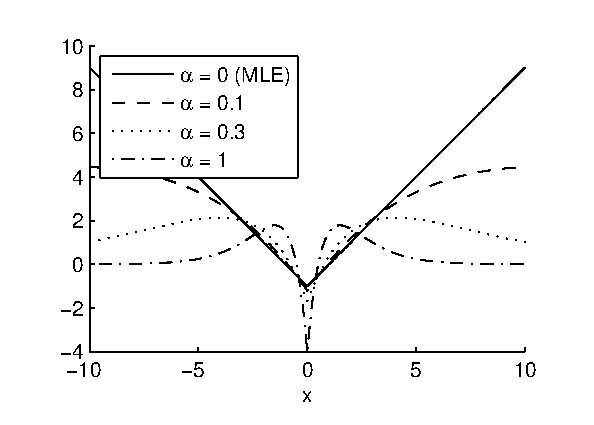
\epsfig{file=Laplace-IF-lambda.eps, height=2in} 
	\\
	$\mathrm{IF}(x;T_{\mathfrak{R}_\alpha},\mu = 0) $ při $\lambda = 1$ známém
	&&
	$\mathrm{IF}(x;T_{\mathfrak{R}_\alpha},\lambda = 1)$ při $\mu = 0$ známém
	\\
\end{tabular}
\caption{Influenční funkce {\mRao}ů pro Laplaceovo rozdělení}
\end{center}
\label{figJK:laplace-if}
\end{figure}

\noindent Z \eqref{IF-laplace-mu} a \eqref{IF-laplace-lambda} vidíme, že jsou obě influenční funkce pro $\alpha>0$ omezené, tedy B-robustní a navíc pro obě funkce platí

\begin{equation}
	\lim_{|x| \rightarrow \infty} \mathrm{IF}(x;T_{\mathfrak{R}_\alpha},\cdot) = 0.
\end{equation}
 
\noindent Nemáme sice konečný bod zamítání $\rho^*$, ale influenční funkce se alespoň limitně blíží s rostoucím $x$ k nule. Tato konvergence je rychlejší s rostoucím $\alpha$ kvůli členu $e^{-\alpha x}$, který se vyskytuje v obou funkcích.


